\documentclass{exam}

%%%%%%%%%%%%%%%%%% PACKAGES %%%%%%%%%%%%%%%%%%%%%%%%

\usepackage{amsmath}
\usepackage{amsfonts}
\usepackage{tcolorbox}
\usepackage{tikz,tkz-euclide,tikz-3dplot}

%%%%%%%%%%%%%%%%%%%%%% MARGINS%% %%%%%%%%%%%%%%%%%%%

\extrawidth{.5in}
\extraheadheight{-.25in}
\extrafootheight{-.25in}

%%%%%%%%%%%%%%%%%% HEADER AND FOOTER %%%%%%%%%%%%%%%

\pagestyle{headandfoot}
\firstpageheadrule
\runningheadrule
\firstpageheader{\S3.EF Review}{}{AP Precalc\\Mr. Carey}
\runningheader{\S3.EF Review}{}{Mr. Carey}
\firstpagefooter{}{}{}
\runningfooter{ }{\thepage}{ }

%%%%%%%%%%%%%%%%%% DOCUMENT CONTENTS %%%%%%%%%%%%%%%

\begin{document}

%%%%%%%%%%%%%%%%%%%%%%%%%%%%%%%%%%%%%%%%%%%%%%%%%%%%

\section*{3.E - Trigonometric Identities and Equations}\label{sec:trig-identities}
\subsection*{Fundamental Identities}

\begin{tcolorbox}[title=Recall: \textit{Fundamental Trigonometric Identities},title filled,colframe=black,sharpish corners,width=\linewidth]
    \begin{minipage}[t]{.45\linewidth}

        \begin{center}
            \textbf{Pythagorean Identities}
        \end{center}
        \[\sin^2\theta+\cos^2\theta=1\]
        \[\tan^2\theta+1=\sec^2\theta\]
        \[1+\cot^2\theta=\csc^2\theta\]
    \end{minipage}
    \hfil
    \begin{minipage}[t]{.45\linewidth}
        \begin{center}
            \textbf{Cofunction Identities}
        \end{center}
        \[\sin\left(\frac{\pi}{2}-\theta\right)=\cos\theta\]
        \[\cos\left(\frac{\pi}{2}-\theta\right)=\sin\theta\]
    \end{minipage}

    \vspace{.2in}

    \begin{minipage}[t]{.45\linewidth}
        \begin{center}
            \textbf{Sum and Difference Identities}
        \end{center}
        \[\sin(\alpha\pm\beta)=\sin\alpha\cos\beta\pm\cos\alpha\sin\beta\]
        \[\cos(\alpha\pm\beta)=\cos\alpha\cos\beta\mp\sin\alpha\sin\beta\]
    \end{minipage}
    \hfil
    \begin{minipage}[t]{.45\linewidth}
        \begin{center}
            \textbf{Even/Odd Identities}
        \end{center}
        \[\sin(-\theta)=-\sin\theta\]
        \[\cos(-\theta)=\cos\theta\]
        \[\tan(-\theta)=-\tan\theta\]
    \end{minipage}

    \vspace{.2in}

    \begin{minipage}[t]{.45\linewidth}
        \begin{center}
            \textbf{Double Angle Identities}
        \end{center}
        \[\sin(2\theta)=2\sin\theta\cos\theta\]
        \[\cos(2\theta)=\cos^2\theta-\sin^2\theta\]
        \[\tan(2\theta)=\frac{2\tan\theta}{1-\tan^2\theta}\]
    \end{minipage}
    \hfil
    \begin{minipage}[t]{.45\linewidth}
        \begin{center}
            \textbf{Power Reducing Identities}
        \end{center}
        \[\sin^2\theta=\frac{1-\cos2\theta}{2}\]
        \[\cos^2\theta=\frac{1+\cos2\theta}{2}\]
        \[\tan^2\theta=\frac{1-\cos2\theta}{1+\cos2\theta}\]
    \end{minipage}



\end{tcolorbox}

\subsection*{Proving Identities}
Recall, to prove an identity, we start with one side of the equation and manipulate it until it looks like the other side. 

\begin{questions}
    \begin{minipage}{.45\linewidth}
        \question $\displaystyle\frac{\sin\theta}{1+\cos\theta}=\frac{1-\cos\theta}{\sin\theta}$    
    \end{minipage}
    \hfill
    \begin{minipage}{.45\linewidth}
        \question $\displaystyle\frac{\sec^2\theta-1}{\sec^2\theta}=\sin^2\theta$    
    \end{minipage}

    \vspace{\stretch{1}}

    \newpage

    \begin{minipage}{.45\linewidth}
        \question $\displaystyle\frac{1}{1-\sin x}+\frac{1}{1+\sin x}=2\sec^2 x$    
    \end{minipage}
    \hfill
    \begin{minipage}{.45\linewidth}
        \question $\displaystyle\left(\tan^2\theta+1\right)\left(\cos^2\theta-1\right)=-\tan^2 \theta$    
    \end{minipage}
    
    \vspace{\stretch{1}}

    \begin{minipage}{.45\linewidth}
        \question $\displaystyle\tan^3 x+1=(\tan x+1)(\sec^2 x-\tan x)$    
    \end{minipage}
    \hfill
    \begin{minipage}{.45\linewidth}
        \question $\displaystyle\sin^3 x\cos^4 x=\left(\cos^4 x-\cos^6 x\right)\sin x$    
    \end{minipage}
    
    \vspace{\stretch{1}}

    \begin{minipage}{.45\linewidth}
        \question $\displaystyle\cos^ 4\theta-\sin^4 \theta=\cos2\theta$    
    \end{minipage}
    \hfill
    \begin{minipage}{.45\linewidth}
        \question $\displaystyle\csc(2x)=\frac{\sec x}{2\sin x}$    
    \end{minipage}
    
    \vspace{\stretch{1}}
\end{questions}

\newpage

\subsection*{Solving Equations}

For each of the following, solve the equation and list all solutions on the interval $[0,2\pi)$.
\begin{questions}
    \begin{minipage}{.45\linewidth}
        \question $\displaystyle2\sin3\theta=-\sqrt{3}$    
    \end{minipage}
    \hfill
    \begin{minipage}{.45\linewidth}
        \question $\displaystyle2\cos^2 \theta+\cos \theta-1=0$    
    \end{minipage}

    \vspace{\stretch{1}}

    \begin{minipage}{.45\linewidth}
        \question $\displaystyle\sin\theta=\sqrt{3}\cos\theta$    
    \end{minipage}
    \hfill
    \begin{minipage}{.45\linewidth}
        \question $\displaystyle\frac{\sin2x}{\cos x}-1=0$    
    \end{minipage}

    \vspace{\stretch{1}}

    \begin{minipage}{.45\linewidth}
        \question $\displaystyle\sec x+\tan x=1$
    \end{minipage}
    \hfill
    \begin{minipage}{.45\linewidth}
        \question $\displaystyle\cos2\theta-\sin^2\theta=\cos^2\theta+3\cos\theta$    
    \end{minipage}

    \vspace{\stretch{1}}

    
\end{questions}

\newpage

\subsection*{Other Problems}
Using identities, and without the use of a calculator, solve the following problems. Your answers should be exact values.
\begin{questions}
    \question $\sin(75^\circ)$

    \vspace{\stretch{1}}

    \question $\displaystyle\cos\left(\frac{5\pi}{12}\right)$

    \vspace{\stretch{1}}

    \question Given $\displaystyle\sin\theta=\frac{5}{14}$ and $\theta$ is in Quadrant II, find $\cos2\theta$.

    \vspace{\stretch{1}}

    \question Given that $\theta=-105^\circ$, find the exact values of sine, cosine, and tangent of $\theta$.

    \vspace{\stretch{1}}
\end{questions}

\newpage

\section*{3.F - Polar Coordinates and Equations}\label{sec:polar-coordinates}
\subsection*{Converting Between Rectangular and Polar Coordinates}
\begin{tcolorbox}[title=Recall: \textit{Converting Between Rectangular and Polar Coordinates},title filled,colframe=black,sharpish corners,width=\linewidth]
    \begin{minipage}[t]{.45\linewidth}

        \begin{center}
            \textbf{Rectangular to Polar}
        \end{center}
        \[r=\sqrt{x^2+y^2}\]
        \[\theta=\arctan\left(\frac{y}{x}\right)\]
    \end{minipage}
    \hfil
    \begin{minipage}[t]{.45\linewidth}
        \begin{center}
            \textbf{Polar to Rectangular}
        \end{center}
        \[x=r\cos\theta\]
        \[y=r\sin\theta\]
    \end{minipage}

\end{tcolorbox}

\noindent Convert each of the following points to rectangular coordinates.
\begin{questions}
    \begin{minipage}{.3\linewidth}
        \question $(3,\pi/6)$    
    \end{minipage}
    \hfill
    \begin{minipage}{.3\linewidth}
        \question $(4,7\pi/4)$    
    \end{minipage}
    \hfill
    \begin{minipage}{.3\linewidth}
        \question $(2,5\pi/3)$    
    \end{minipage}

    \vspace{\stretch{1}}

    \begin{minipage}{.3\linewidth}
        \question $(-3,5\pi/6)$    
    \end{minipage}
    \hfill
    \begin{minipage}{.3\linewidth}
        \question $(-4,-7\pi/6)$    
    \end{minipage}
    \hfill
    \begin{minipage}{.3\linewidth}
        \question $(0,1\pi/3)$    
    \end{minipage}

    \vspace{\stretch{1}}

\end{questions}

\noindent Convert each of the following points to polar coordinates.
\begin{questions}
    \begin{minipage}{.3\linewidth}
        \question $(3,4)$    
    \end{minipage}
    \hfill
    \begin{minipage}{.3\linewidth}
        \question $(-3,4)$    
    \end{minipage}
    \hfill
    \begin{minipage}{.3\linewidth}
        \question $(-3,-4)$    
    \end{minipage}

    \vspace{\stretch{1}}

    \begin{minipage}{.3\linewidth}
        \question $(2\sqrt{3},-2)$    
    \end{minipage}
    \hfill
    \begin{minipage}{.3\linewidth}
        \question $(-1,\sqrt{3})$    
    \end{minipage}
    \hfill
    \begin{minipage}{.3\linewidth}
        \question $(8,0)$    
    \end{minipage}

    \vspace{\stretch{1}}

\end{questions}

\newpage

\subsection*{Converting Equations}
\noindent Convert each of the following equations from rectangular to polar form.
\begin{questions}
    \begin{minipage}{.45\linewidth}
        \question $y^2=-x^2+16$    
    \end{minipage}
    \hfill
    \begin{minipage}{.45\linewidth}
        \question $xy=-(x-2)^2$    
    \end{minipage}

    \vspace{\stretch{1}}

\end{questions}

\noindent Convert each of the following equations from polar to rectangular form.
\begin{questions}
    \begin{minipage}{.45\linewidth}
        \question $r=3$    
    \end{minipage}
    \hfill
    \begin{minipage}{.45\linewidth}
        \question $r=2\sec\theta$    
    \end{minipage}

    \vspace{\stretch{1}}

    \begin{minipage}{.45\linewidth}
        \question $\theta=-\frac{11\pi}{6}$    
    \end{minipage}
    \hfill
    \begin{minipage}{.45\linewidth}
        \question $r=-2\sin\theta$    
    \end{minipage}

    \vspace{\stretch{1}}

    \begin{minipage}{.45\linewidth}
        \question $r=5\sin\theta\cos\theta$
    \end{minipage}
    \hfill
    \begin{minipage}{.45\linewidth}
            
    \end{minipage}

    \vspace{\stretch{1}}

    
\end{questions}

\newpage

\subsection*{Graphing Polar Equations}
Sketch a graph of the given polar functions. Confirm your answer with a calculator or Desmos.com.
\begin{questions}
    \begin{minipage}[t]{.45\linewidth}
        \question $r=3\cos\theta$   
        
        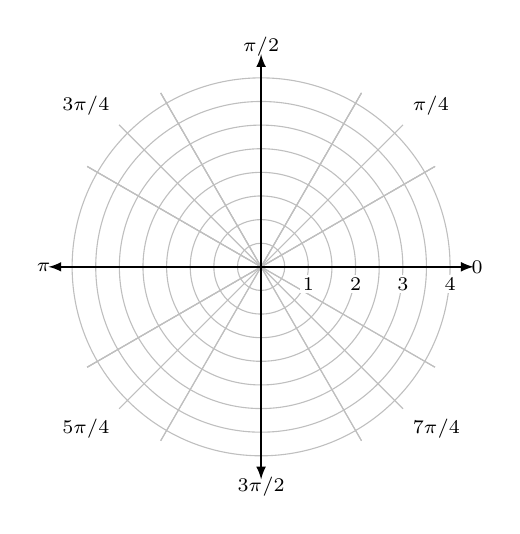
\begin{tikzpicture}[scale=.6]
             

            % Draw the lines at multiples of pi/6
            \foreach \ang in {0,...,31} {
                \draw [lightgray] (0,0) -- (\ang * 180 / 6:4.25);
            }
            
            % Add the labels at multiples of pi/4
            \foreach \ang/\lab/\dir in {
            0/0/right,
            1/{\pi/4}/{above right},
            2/{\pi/2}/above,
            3/{3\pi/4}/{above left},
            4/{\pi}/left,
            5/{5\pi/4}/{below left},
            7/{7\pi/4}/{below right},
            6/{3\pi/2}/below} {
            \draw [lightgray] (0,0) -- (\ang * 180 / 4:4.25);
            \node [fill=white] at (\ang * 180 / 4:4.25) [\dir] {\scriptsize $\lab$};
            }
            
            % Concentric circles and radius labels
            \foreach \s in  {1, 2, 3, 4} {
            \draw [lightgray] (0,0) circle (\s - 0.5);
            \draw [lightgray] (0,0) circle (\s);
            \node [fill=white] at (\s, 0) [below=1mm,inner sep=1pt] {\scriptsize $\s$};
            }

            \draw[latex-latex,semithick](-4.5,0)--(4.5,0);
            \draw[latex-latex,semithick](0,-4.5)--(0,4.5); 

            %\draw[domain=0:6.29,samples=200,smooth,-latex,thick,] plot ({deg(\x)}:{3*cos(\x r)});

        \end{tikzpicture}

    \end{minipage}
    \hfill
    \begin{minipage}[t]{.45\linewidth}
        \question $r=-2\sin\theta$  
        
        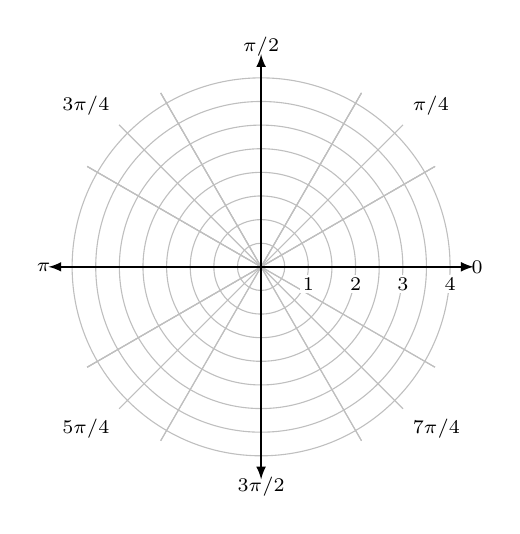
\begin{tikzpicture}[scale=.6]
             

            % Draw the lines at multiples of pi/6
            \foreach \ang in {0,...,31} {
                \draw [lightgray] (0,0) -- (\ang * 180 / 6:4.25);
            }
            
            % Add the labels at multiples of pi/4
            \foreach \ang/\lab/\dir in {
            0/0/right,
            1/{\pi/4}/{above right},
            2/{\pi/2}/above,
            3/{3\pi/4}/{above left},
            4/{\pi}/left,
            5/{5\pi/4}/{below left},
            7/{7\pi/4}/{below right},
            6/{3\pi/2}/below} {
            \draw [lightgray] (0,0) -- (\ang * 180 / 4:4.25);
            \node [fill=white] at (\ang * 180 / 4:4.25) [\dir] {\scriptsize $\lab$};
            }
            
            % Concentric circles and radius labels
            \foreach \s in  {1, 2, 3, 4} {
            \draw [lightgray] (0,0) circle (\s - 0.5);
            \draw [lightgray] (0,0) circle (\s);
            \node [fill=white] at (\s, 0) [below=1mm,inner sep=1pt] {\scriptsize $\s$};
            }

            \draw[latex-latex,semithick](-4.5,0)--(4.5,0);
            \draw[latex-latex,semithick](0,-4.5)--(0,4.5); 

            %\draw[domain=0:6.29,samples=200,smooth,-latex,thick,] plot ({deg(\x)}:{-2*sin(\x r)});

        \end{tikzpicture}
    \end{minipage}

    \vspace{\stretch{1}}

    \begin{minipage}[t]{.45\linewidth}
        \question $r=4\sin2\theta$   
        
        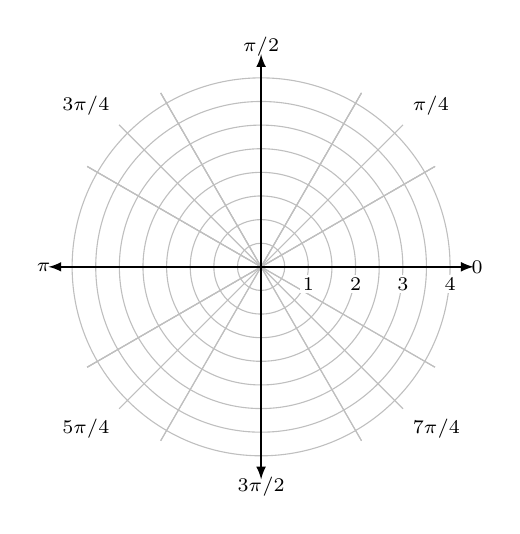
\begin{tikzpicture}[scale=.6]
             

            % Draw the lines at multiples of pi/6
            \foreach \ang in {0,...,31} {
                \draw [lightgray] (0,0) -- (\ang * 180 / 6:4.25);
            }
            
            % Add the labels at multiples of pi/4
            \foreach \ang/\lab/\dir in {
            0/0/right,
            1/{\pi/4}/{above right},
            2/{\pi/2}/above,
            3/{3\pi/4}/{above left},
            4/{\pi}/left,
            5/{5\pi/4}/{below left},
            7/{7\pi/4}/{below right},
            6/{3\pi/2}/below} {
            \draw [lightgray] (0,0) -- (\ang * 180 / 4:4.25);
            \node [fill=white] at (\ang * 180 / 4:4.25) [\dir] {\scriptsize $\lab$};
            }
            
            % Concentric circles and radius labels
            \foreach \s in  {1, 2, 3, 4} {
            \draw [lightgray] (0,0) circle (\s - 0.5);
            \draw [lightgray] (0,0) circle (\s);
            \node [fill=white] at (\s, 0) [below=1mm,inner sep=1pt] {\scriptsize $\s$};
            }

            \draw[latex-latex,semithick](-4.5,0)--(4.5,0);
            \draw[latex-latex,semithick](0,-4.5)--(0,4.5); 

            %\draw[domain=0:6.29,samples=200,smooth,-latex,thick,] plot ({deg(\x)}:{3*cos(\x r)});

        \end{tikzpicture}

    \end{minipage}
    \hfill
    \begin{minipage}[t]{.45\linewidth}
        \question $r=1+3\cos\theta$  
        
        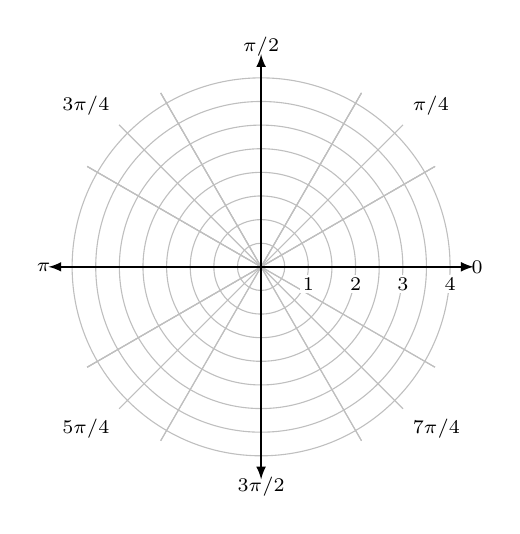
\begin{tikzpicture}[scale=.6]
             

            % Draw the lines at multiples of pi/6
            \foreach \ang in {0,...,31} {
                \draw [lightgray] (0,0) -- (\ang * 180 / 6:4.25);
            }
            
            % Add the labels at multiples of pi/4
            \foreach \ang/\lab/\dir in {
            0/0/right,
            1/{\pi/4}/{above right},
            2/{\pi/2}/above,
            3/{3\pi/4}/{above left},
            4/{\pi}/left,
            5/{5\pi/4}/{below left},
            7/{7\pi/4}/{below right},
            6/{3\pi/2}/below} {
            \draw [lightgray] (0,0) -- (\ang * 180 / 4:4.25);
            \node [fill=white] at (\ang * 180 / 4:4.25) [\dir] {\scriptsize $\lab$};
            }
            
            % Concentric circles and radius labels
            \foreach \s in  {1, 2, 3, 4} {
            \draw [lightgray] (0,0) circle (\s - 0.5);
            \draw [lightgray] (0,0) circle (\s);
            \node [fill=white] at (\s, 0) [below=1mm,inner sep=1pt] {\scriptsize $\s$};
            }

            \draw[latex-latex,semithick](-4.5,0)--(4.5,0);
            \draw[latex-latex,semithick](0,-4.5)--(0,4.5); 

            %\draw[domain=0:6.29,samples=200,smooth,-latex,thick,] plot ({deg(\x)}:{-2*sin(\x r)});

        \end{tikzpicture}
    \end{minipage}

    \vspace{\stretch{1}}

    \newpage

    \begin{minipage}[t]{.45\linewidth}
        \question $r=-3-3\sin\theta$   
        
        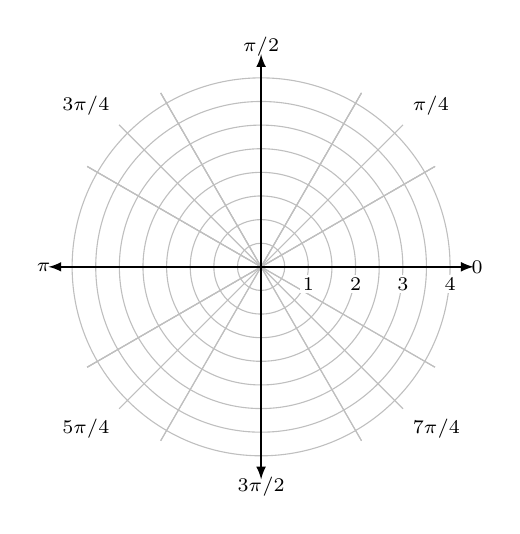
\begin{tikzpicture}[scale=.6]
             

            % Draw the lines at multiples of pi/6
            \foreach \ang in {0,...,31} {
                \draw [lightgray] (0,0) -- (\ang * 180 / 6:4.25);
            }
            
            % Add the labels at multiples of pi/4
            \foreach \ang/\lab/\dir in {
            0/0/right,
            1/{\pi/4}/{above right},
            2/{\pi/2}/above,
            3/{3\pi/4}/{above left},
            4/{\pi}/left,
            5/{5\pi/4}/{below left},
            7/{7\pi/4}/{below right},
            6/{3\pi/2}/below} {
            \draw [lightgray] (0,0) -- (\ang * 180 / 4:4.25);
            \node [fill=white] at (\ang * 180 / 4:4.25) [\dir] {\scriptsize $\lab$};
            }
            
            % Concentric circles and radius labels
            \foreach \s in  {1, 2, 3, 4} {
            \draw [lightgray] (0,0) circle (\s - 0.5);
            \draw [lightgray] (0,0) circle (\s);
            \node [fill=white] at (\s, 0) [below=1mm,inner sep=1pt] {\scriptsize $\s$};
            }

            \draw[latex-latex,semithick](-4.5,0)--(4.5,0);
            \draw[latex-latex,semithick](0,-4.5)--(0,4.5); 

            %\draw[domain=0:6.29,samples=200,smooth,-latex,thick,] plot ({deg(\x)}:{3*cos(\x r)});

        \end{tikzpicture}

    \end{minipage}
    \hfill
    \begin{minipage}[t]{.45\linewidth}
        \question $r=-3\cos(3\theta)$  
        
        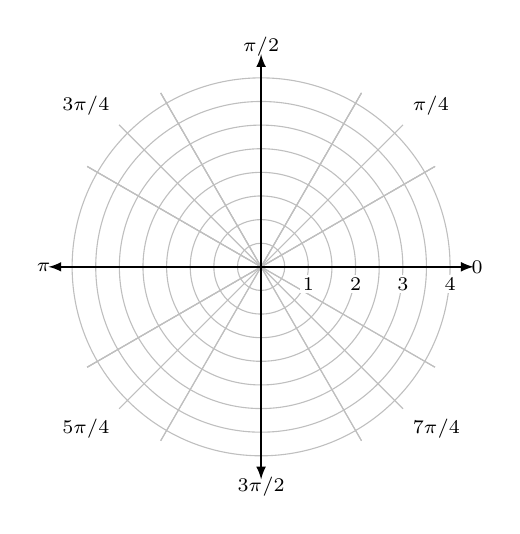
\begin{tikzpicture}[scale=.6]
             

            % Draw the lines at multiples of pi/6
            \foreach \ang in {0,...,31} {
                \draw [lightgray] (0,0) -- (\ang * 180 / 6:4.25);
            }
            
            % Add the labels at multiples of pi/4
            \foreach \ang/\lab/\dir in {
            0/0/right,
            1/{\pi/4}/{above right},
            2/{\pi/2}/above,
            3/{3\pi/4}/{above left},
            4/{\pi}/left,
            5/{5\pi/4}/{below left},
            7/{7\pi/4}/{below right},
            6/{3\pi/2}/below} {
            \draw [lightgray] (0,0) -- (\ang * 180 / 4:4.25);
            \node [fill=white] at (\ang * 180 / 4:4.25) [\dir] {\scriptsize $\lab$};
            }
            
            % Concentric circles and radius labels
            \foreach \s in  {1, 2, 3, 4} {
            \draw [lightgray] (0,0) circle (\s - 0.5);
            \draw [lightgray] (0,0) circle (\s);
            \node [fill=white] at (\s, 0) [below=1mm,inner sep=1pt] {\scriptsize $\s$};
            }

            \draw[latex-latex,semithick](-4.5,0)--(4.5,0);
            \draw[latex-latex,semithick](0,-4.5)--(0,4.5); 

            %\draw[domain=0:6.29,samples=200,smooth,-latex,thick,] plot ({deg(\x)}:{-2*sin(\x r)});

        \end{tikzpicture}
    \end{minipage}

    \vspace{\stretch{2}}

    



\end{questions}

\noindent Given the graph of a polar curve, write the equation $r=f(\theta)$ that describes it. There may be multiple answers.

\begin{questions}
    \begin{minipage}[t]{.45\linewidth}
        \question \hfill
        
        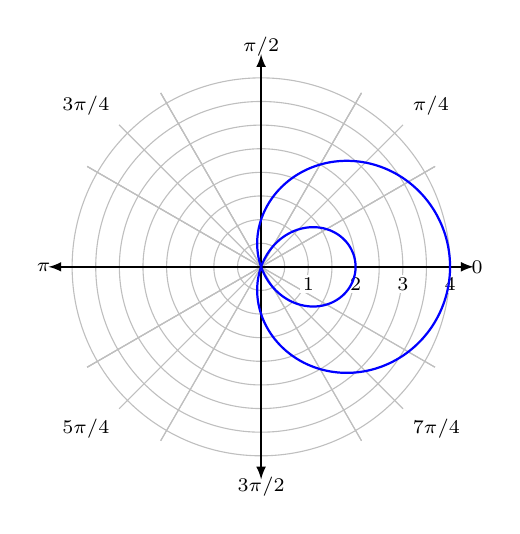
\begin{tikzpicture}[scale=.6]
             

            % Draw the lines at multiples of pi/6
            \foreach \ang in {0,...,31} {
                \draw [lightgray] (0,0) -- (\ang * 180 / 6:4.25);
            }
            
            % Add the labels at multiples of pi/4
            \foreach \ang/\lab/\dir in {
            0/0/right,
            1/{\pi/4}/{above right},
            2/{\pi/2}/above,
            3/{3\pi/4}/{above left},
            4/{\pi}/left,
            5/{5\pi/4}/{below left},
            7/{7\pi/4}/{below right},
            6/{3\pi/2}/below} {
            \draw [lightgray] (0,0) -- (\ang * 180 / 4:4.25);
            \node [fill=white] at (\ang * 180 / 4:4.25) [\dir] {\scriptsize $\lab$};
            }
            
            % Concentric circles and radius labels
            \foreach \s in  {1, 2, 3, 4} {
            \draw [lightgray] (0,0) circle (\s - 0.5);
            \draw [lightgray] (0,0) circle (\s);
            \node [fill=white] at (\s, 0) [below=1mm,inner sep=1pt] {\scriptsize $\s$};
            }

            \draw[latex-latex,semithick](-4.5,0)--(4.5,0);
            \draw[latex-latex,semithick](0,-4.5)--(0,4.5); 

            \draw[domain=0:6.29,samples=300,smooth,thick,blue] plot ({deg(\x)}:{1+3*cos(\x r)});

        \end{tikzpicture}

    \end{minipage}
    \hfill
    \begin{minipage}[t]{.45\linewidth}
        \question \hfill

        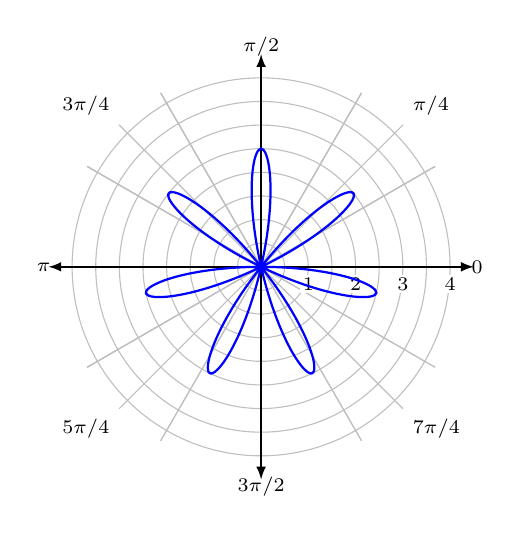
\begin{tikzpicture}[scale=.6]
             

            % Draw the lines at multiples of pi/6
            \foreach \ang in {0,...,31} {
                \draw [lightgray] (0,0) -- (\ang * 180 / 6:4.25);
            }
            
            % Add the labels at multiples of pi/4
            \foreach \ang/\lab/\dir in {
            0/0/right,
            1/{\pi/4}/{above right},
            2/{\pi/2}/above,
            3/{3\pi/4}/{above left},
            4/{\pi}/left,
            5/{5\pi/4}/{below left},
            7/{7\pi/4}/{below right},
            6/{3\pi/2}/below} {
            \draw [lightgray] (0,0) -- (\ang * 180 / 4:4.25);
            \node [fill=white] at (\ang * 180 / 4:4.25) [\dir] {\scriptsize $\lab$};
            }
            
            % Concentric circles and radius labels
            \foreach \s in  {1, 2, 3, 4} {
            \draw [lightgray] (0,0) circle (\s - 0.5);
            \draw [lightgray] (0,0) circle (\s);
            \node [fill=white] at (\s, 0) [below=1mm,inner sep=1pt] {\scriptsize $\s$};
            }

            \draw[latex-latex,semithick](-4.5,0)--(4.5,0);
            \draw[latex-latex,semithick](0,-4.5)--(0,4.5); 

            \draw[domain=0:6.29,samples=300,smooth,thick,blue] plot ({deg(\x)}:{-2.5*sin(7*(\x r))});

        \end{tikzpicture}
    \end{minipage}

    \vspace{\stretch{1}}

    \newpage

    \begin{minipage}[t]{.45\linewidth}
        \question \hfill
        
        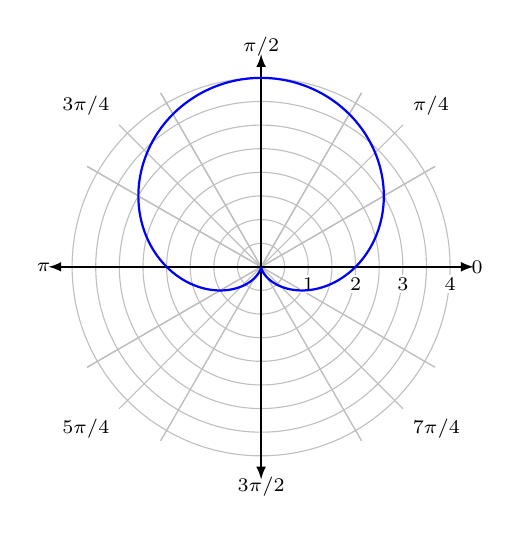
\begin{tikzpicture}[scale=.6]
             

            % Draw the lines at multiples of pi/6
            \foreach \ang in {0,...,31} {
                \draw [lightgray] (0,0) -- (\ang * 180 / 6:4.25);
            }
            
            % Add the labels at multiples of pi/4
            \foreach \ang/\lab/\dir in {
            0/0/right,
            1/{\pi/4}/{above right},
            2/{\pi/2}/above,
            3/{3\pi/4}/{above left},
            4/{\pi}/left,
            5/{5\pi/4}/{below left},
            7/{7\pi/4}/{below right},
            6/{3\pi/2}/below} {
            \draw [lightgray] (0,0) -- (\ang * 180 / 4:4.25);
            \node [fill=white] at (\ang * 180 / 4:4.25) [\dir] {\scriptsize $\lab$};
            }
            
            % Concentric circles and radius labels
            \foreach \s in  {1, 2, 3, 4} {
            \draw [lightgray] (0,0) circle (\s - 0.5);
            \draw [lightgray] (0,0) circle (\s);
            \node [fill=white] at (\s, 0) [below=1mm,inner sep=1pt] {\scriptsize $\s$};
            }

            \draw[latex-latex,semithick](-4.5,0)--(4.5,0);
            \draw[latex-latex,semithick](0,-4.5)--(0,4.5); 

            \draw[domain=0:6.29,samples=300,smooth,thick,blue] plot ({deg(\x)}:{2+2*sin(\x r)});

        \end{tikzpicture}

    \end{minipage}
    \hfill
    \begin{minipage}[t]{.45\linewidth}
        \question \hfill

        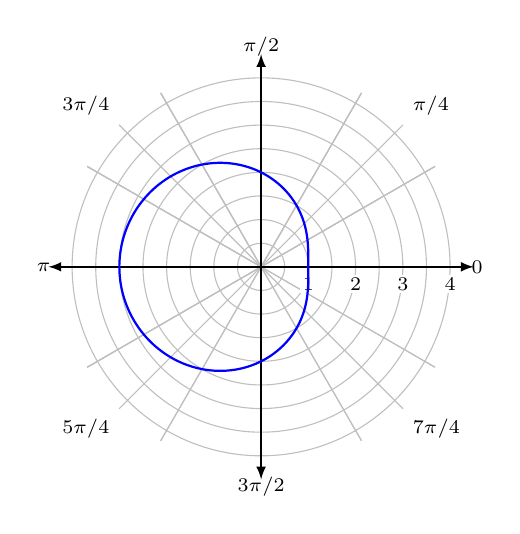
\begin{tikzpicture}[scale=.6]
             

            % Draw the lines at multiples of pi/6
            \foreach \ang in {0,...,31} {
                \draw [lightgray] (0,0) -- (\ang * 180 / 6:4.25);
            }
            
            % Add the labels at multiples of pi/4
            \foreach \ang/\lab/\dir in {
            0/0/right,
            1/{\pi/4}/{above right},
            2/{\pi/2}/above,
            3/{3\pi/4}/{above left},
            4/{\pi}/left,
            5/{5\pi/4}/{below left},
            7/{7\pi/4}/{below right},
            6/{3\pi/2}/below} {
            \draw [lightgray] (0,0) -- (\ang * 180 / 4:4.25);
            \node [fill=white] at (\ang * 180 / 4:4.25) [\dir] {\scriptsize $\lab$};
            }
            
            % Concentric circles and radius labels
            \foreach \s in  {1, 2, 3, 4} {
            \draw [lightgray] (0,0) circle (\s - 0.5);
            \draw [lightgray] (0,0) circle (\s);
            \node [fill=white] at (\s, 0) [below=1mm,inner sep=1pt] {\scriptsize $\s$};
            }

            \draw[latex-latex,semithick](-4.5,0)--(4.5,0);
            \draw[latex-latex,semithick](0,-4.5)--(0,4.5); 

            \draw[domain=0:6.29,samples=300,smooth,thick,blue] plot ({deg(\x)}:{-2-1*cos((\x r))});

        \end{tikzpicture}
    \end{minipage}

    \vspace{\stretch{1}}

\end{questions}

\subsection*{Symmetry}
Find all axes or lines of symmetry for the provided polar functions.

\begin{questions}
    \begin{minipage}{.45\linewidth}
        \question $r=3\sin\theta$    
    \end{minipage}
    \hfill
    \begin{minipage}{.45\linewidth}
        \question $r=4\cos2\theta$    
    \end{minipage}

    \vspace{\stretch{1}}

    
\end{questions}


\newpage


\subsection*{Rates of Change}
Find the average rate of change of the given polar functions over the given interval $[a,b]$. Round to 3 decimal places.

\begin{questions}
    \begin{minipage}{.45\linewidth}
        \question $\displaystyle r=2\sin(3\pi\theta)$ over $\displaystyle \left[1,\frac{7}{6}\right]$    
    \end{minipage}
    \hfill
    \begin{minipage}{.45\linewidth}
        \question $\displaystyle r=2\cos\left(\frac{5}{3}\theta\right)+3$ over $\displaystyle \left[-\frac{12\pi}{5},-\frac{9\pi}{4}\right]$    
    \end{minipage}

    \vspace{\stretch{1}}

    
\end{questions}

\noindent For each of the following polar functions, determine \textbf{(1)} if $r$ and \textbf{(2)} the distance from the origin are increasing, decreasing, or neither at the given value of $\theta$.

\begin{questions}
    \begin{minipage}{.45\linewidth}
        \question $r=2\sin\theta$ at $\theta=\pi/4$    
    \end{minipage}
    \hfill
    \begin{minipage}{.45\linewidth}
        \question $r=3\cos\theta$ at $\theta=3\pi/2$    
    \end{minipage}

    \vspace{\stretch{1}}

    \begin{minipage}{.45\linewidth}
        \question $r=4\sin2\theta$ at $\theta=\pi/6$    
    \end{minipage}
    \hfill
    \begin{minipage}{.45\linewidth}
        \question $r=1+3\cos\theta$ at $\theta=0$    
    \end{minipage}

    \vspace{\stretch{1}}
\end{questions}

    


%%%%%%%%%%%%%%%%%%%%%%%%%%%%%%%%%%%%%%%%%%%%%%%%%%%%

\end{document}